\chapter{Power considerations}
This chapter provides a close look at the power consumption of DWT. Robots need the ability to work for extended periods. Unfortunately, energy technology is slow to progress, with no foreseeable major improvements in the future~\cite{paradiso2005energy}.  We discuss the previous work in energy harvesting and analyze the power consumption of the robot. We also discuss the possibility of energy harvesting. 

\section{Energy harvesting technologies}
A thorough review of energy harvesting in wearable devices is provided in~\cite{paradiso2005energy}. In this section, we will look at potential energy harvesting technologies and try to understand their limitations. 

\textbf{Electromagnetic}. 
RF provides a useful source of wireless energy. In my master's thesis, I explored such wireless power solutions for sensors~\cite{dementyev2013applications}. Commercial UHF (Ultra high frequency) RFID tags can provide enough energy to power a sensor and a microcontroller, as well as use backscatter for communications~\cite{sample2008design}. For example, we demonstrated that  EEG (Electroencephalogram) can be powered with UHF RFID~\cite{dementyev2013wearable}. UHF provides a relatively small amount of energy in the order of microWatts (uW), so duty cycling is usually required. Ambient RF energy from TV broadcast antennas can provide around more than 100 uW~\cite{parks2013wireless} in 10km proximity but requires a large antenna.

NFC (Near-field communications) provide a much more significant amount of energy from milliWatts to Watts. NFC is adapted for phone wireless charging and non-contact payments. We demonstrated that NFC can power small displays~\cite{dementyev2013wirelessly}. NFC does not use radio waves but works as an air-gap transformer between receiver and transmitter coils. As a result,  NFC needs precise alignment and has a maximum range of few centimeters. The range can be increased using resonant coupling~\cite{sample2011analysis}. 

Another way to convert mechanical energy into electrical energy by moving a magnet near a wire. Similar to electric generators, the movement generates a current inside the coil.  There are commercial flashlights which create electrical energy from shaking or cranking. Significant power can be made but requires mechanical input. 

\textbf{Piezo electric}. 
Piezoelectric materials generate electrical energy from strain on their crystalline structure. For example, a microfabricated piezoelectric material can harvest energy when placed on the surface of the heart~\cite{dagdeviren2014conformal}. Placed in solos of the shoes, piezoelectric materials generate electricity for every step~\cite{shenck2001energy}

\textbf{Thermal energy}. When two different metals are sandwiched together, they will produce electricity if there is a temperature gradient. Such device forms a thermoelectric generator. Such generators have been integrated into flexible fabrics ~\cite{kim2014wearable}. 

\textbf{Solar and optical}. 
Solar panels can extract energy from photons proportional to their area and intensity of light.  Hovewhere, solar panels provide significantly less energy indoors. 

\textbf{Battery technology}. Most untethered robots and consumer devices are powered by lithium polymer (LiPo) batteries. This technology provides good energy density and rechargeable chemistry. Since LiPo, there have not been major commercial breakthroughs in battery technology~\cite{van2014rechargeable}, although LiPo energy densities are steadily increasing. Batteries require many factors such as durability, energy density, charge cycles, which has not been fully satisfied with emerging technologies. 

Some of the recent research focused on making solid-state batteries, which have solid electrolyte to allow thinner and safer batteries~\cite{manthiram2017lithium}. Most LiPo batteries use gel or liquid electrolyte, which requires a thick aluminum-backed pouch for sealing and turns into gas when overheated. Another possibility is to use a lithium-oxygen chemical reaction, as oxygen is present in the air, the energy density of the battery is higher~\cite{jung2012improved} 

\textbf{Summary}. 
None of the energy harvesting technologies can power the robot continuously without external setups. The robot has to be powered from a battery.  However, energy harvesting can provide an additional energy source for the batteries.  

\section{Power consumption of Epidermal robots}
\begin{figure}[!b]
\centering
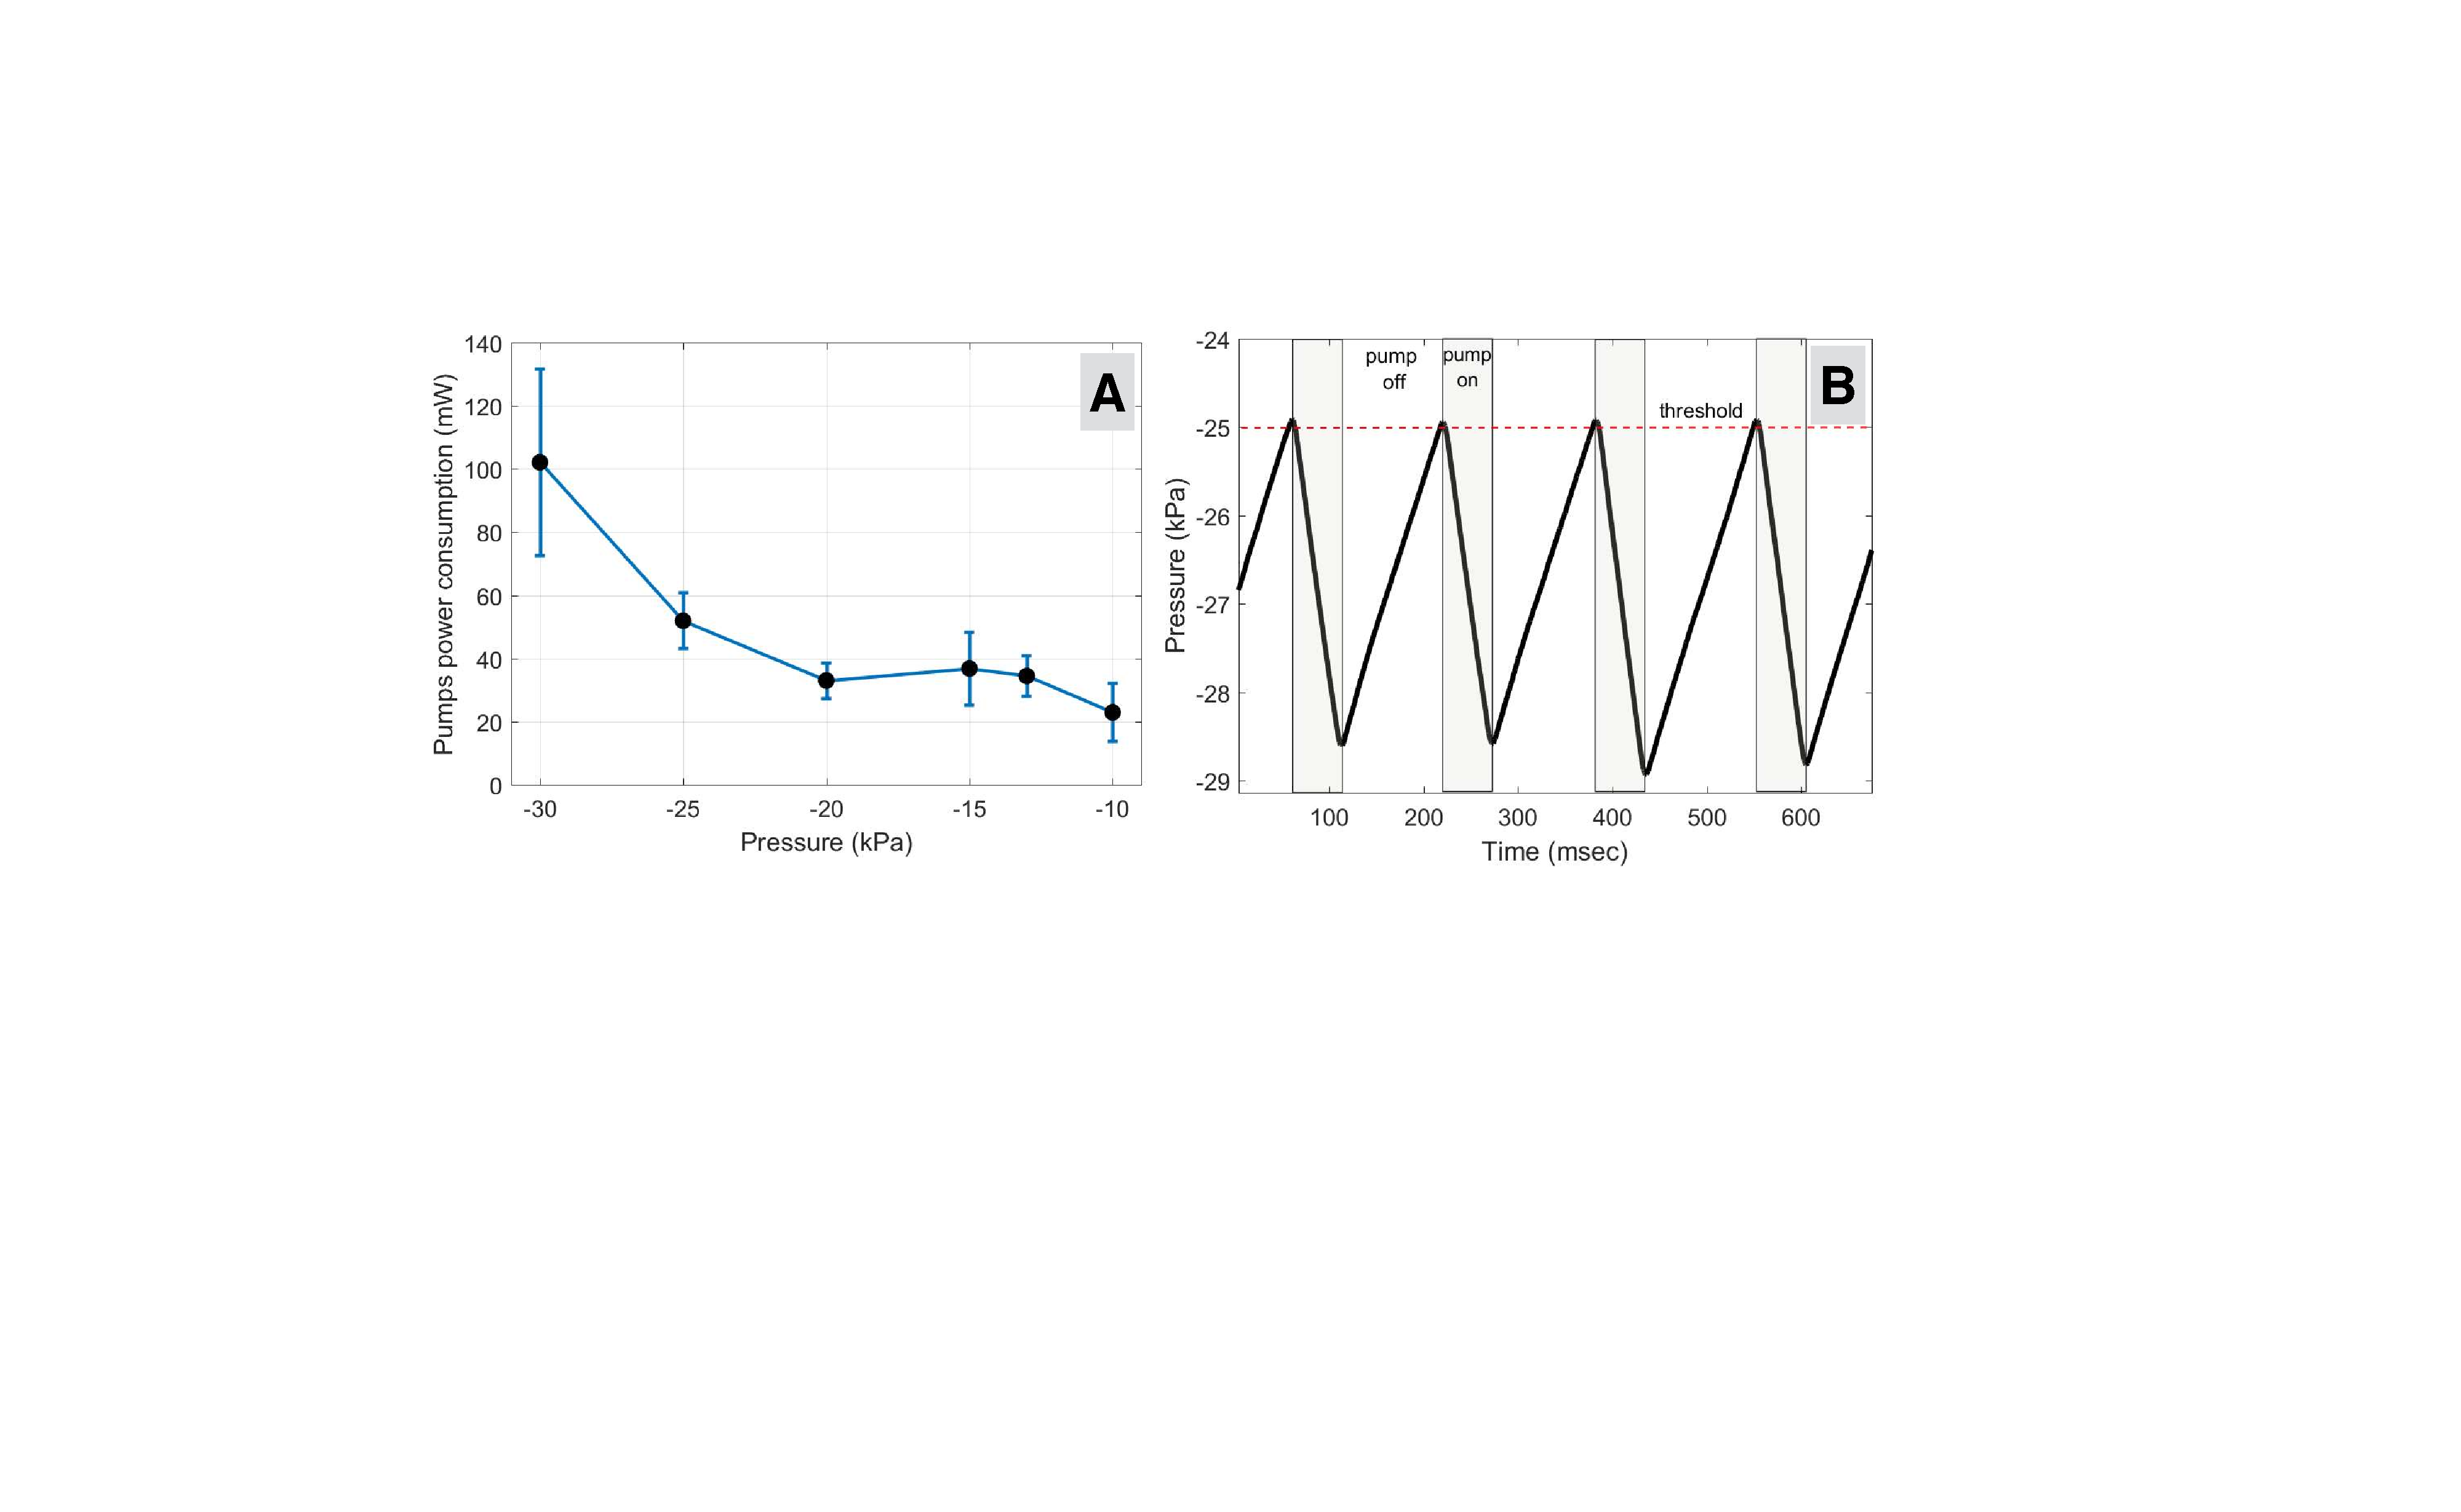
\includegraphics[width=15.0cm]{pictures/chapter3/power_consumption.pdf}
\caption{Power consumption during the adhesion experiment. A)~The power consumption of the pumps required to keep the robot attached to the skin at different vacuum pressures. The pumps were duty cycled by turning on only when vacuum goes under a certain threshold. Overall, the power consumption is an order of magnitude lower than running pumps continuously at 1076mW. B)~Sample pressure data showing duty cycling of the pressure to keep the pressure at the threshold of -25kPa.}
\label{fig:power_consumption}
\end{figure}

Using a digital multimeter (U1252B, Agilent) and average currents over five minute periods, the mean power consumption of the robot during locomotion was found to be 1221mW. A significant part of the power is consumed by the pumps (817mW), and the rest is used by the five motors (404mW). When the robot is statically attached to the skin, the power consumption of the pumps is reduced to 30mW. This significant reduction can be achieved by monitoring the pressure sensors and only activating the pumps when the vacuum pressure drops under -20kPa. Pumps run at a duty cycle of 2\% to 5\% at -20kPa pressure. Fig.~\ref{fig:power_consumption} illustrates the power consumption at different pressures, and shows that -20kPa provides the most vacuum pressure while consuming the least energy. The current for each pressure threshold was measured at five different locations on the forearm. 

To evaluate the feasibility of an untethered version of SkinBot, we built the prototype shown in Figure~\ref{fig:untethered_prototype}. In particular, the PCB that held the original tether was replaced by a custom PCB that contained all the electronics required for operation; 2.4 GHz radio (nRF24L01+, Nordic), an ARM-based microcontroller (ATMSAMD21G, Atmel) and an IMU (MPU6050, Invensense). This version of the robot is powered by a 100mAh lithium polymer battery. The vacuum pumps were also added to the robot, but the torque from unbalanced weight made it unreliable for continuous vertical climbing. The electronics consumed a relatively small amount of energy (28.1mW) even with a 2-way radio transmission at 10Hz. Based on our measurements, the untethered robot could move continuously for around 16 minutes or remain attached to the skin for about 10 hours.

\begin{figure}[!ht]
\centering
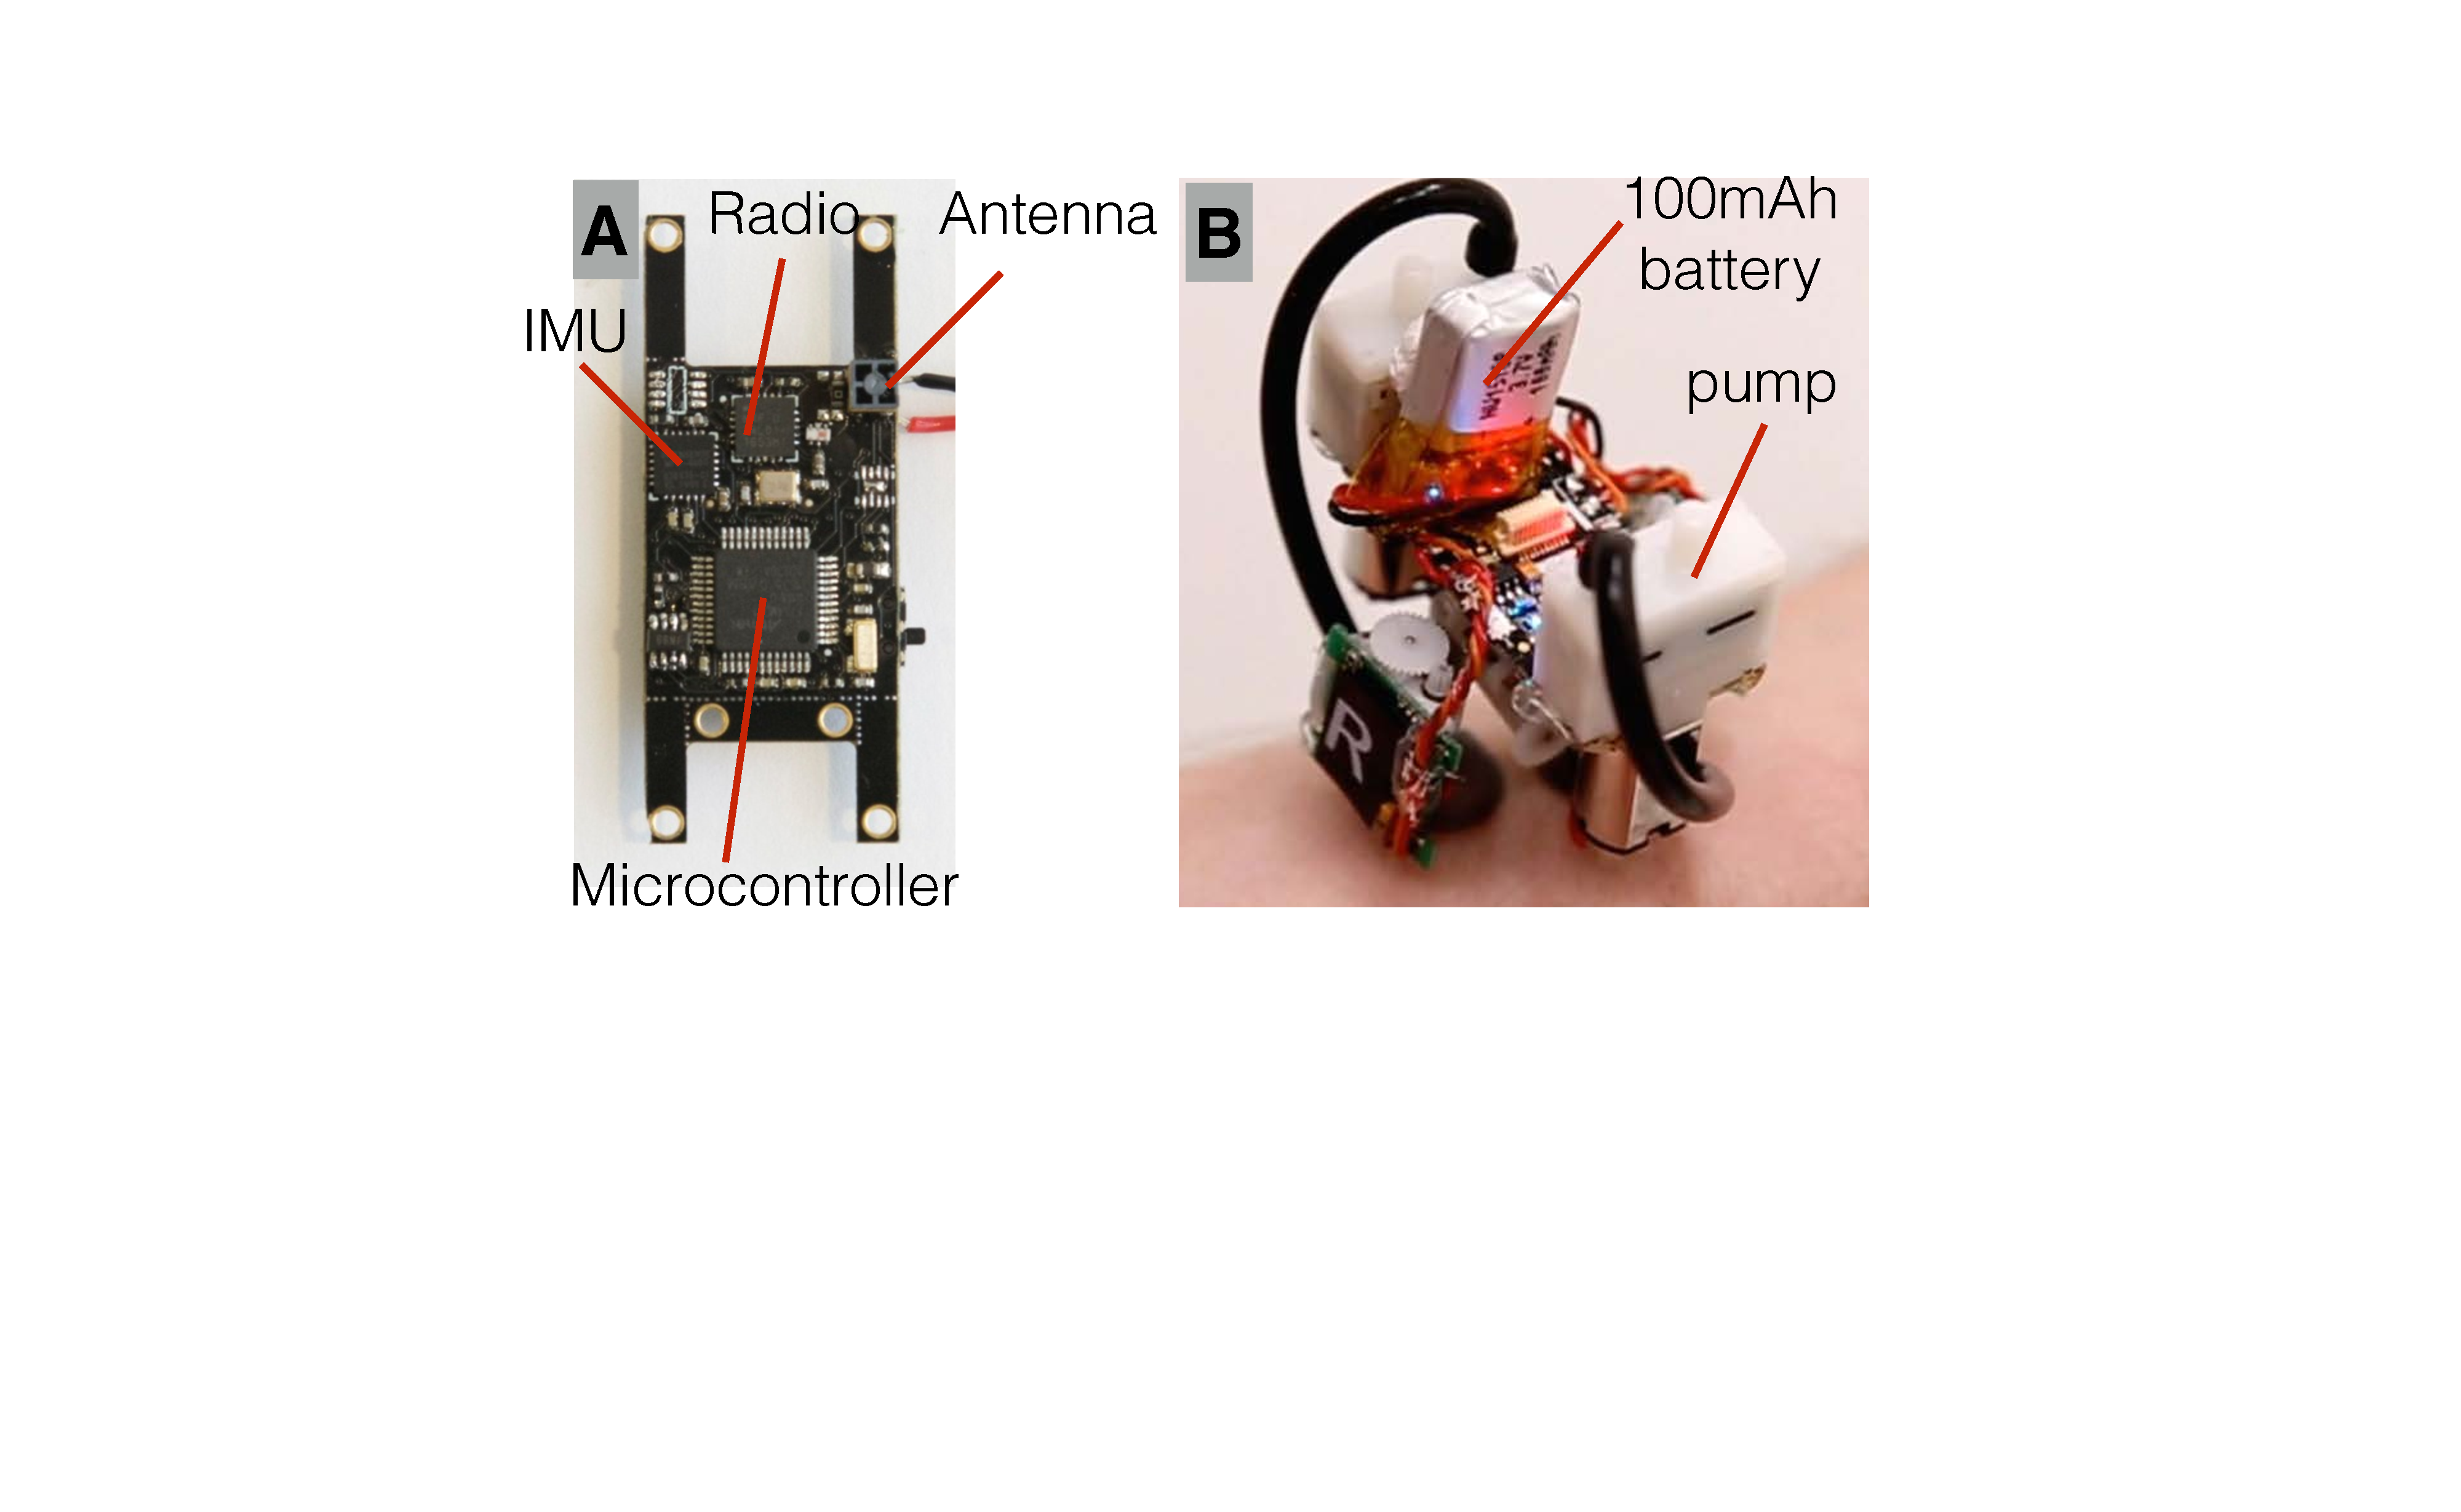
\includegraphics[width=10.0cm]{pictures/chapter3/untethered_prototype.pdf}
\caption{A) Circuit board and B) assembled untethered prototype of SkinBot}
\label{fig:untethered_prototype}
\end{figure}

\section{Power consumption of Rovables}
The Rovables robot works untethered with an on-board LiPo battery. The maximum power consumption is 120.4mA (398mW), which allows for a battery life of 45 minutes with a 100mAh battery. This is the power required with motors on and all systems on (IMU, wireless, encoders). Motors use the most energy: 91.9mA. The encoder's infrared LEDs consume 20mA. The rest of the electronics consume just under 8.5mA. 

Assuming that all systems will not be active all the time, the battery life could be significantly extended. For example, optical encoders can be disabled when motors are not running. 
The device can wirelessly stream data for 11.8 hours if the motors and encoders are off. 




\section{Power analysis}
% Add graph of individual component power consumption. 
%Duty cycling add
This section looks at the power consumption of different subsystems of  DWT robot. The maximum power consumption is given in most cases. It is difficult to generalize the mean power consumption, as power depends on many factors during operation, such as sleep modes and motor torque and speed. 
Also, during normal operation, all the subsystems are duty cycled. 

To better understand the power consumption, it is best to have a realistic scenario. Let us assume that the robot moves for 5 seconds, then stops for 5 seconds to take an image. During movement, the motors, processor, IMU, and encoders are active. When stopped, the radio and camera are active for 100ms to take a picture. This time includes the time for start-up, image taking, and transfer. 

\textbf{Processor}
Modern digital electronics have low power consumption. State-of-the-art ARM-based microcontrollers consume the maximum of 8mA at 64MHz. Although, in the typical application, the average consumption is lower, as the microcontroller is often in the sleep mode, where the power consumption is in the microAmpere (uA) range. 
At a 50\% duty cycle, the power consumption is around 4mA. 

\textbf{Communications}
The power consumption of Bluetooth Low Energy (BLE) radio is about 5.0mA during constant transmission. 

The maximum throughput of BLE is about 171kb/sec. This throughput assumes 244-byte packets are sent at transmission period of 400 ms and 2Mbit physical layer speed. The size of an uncompressed 5-megapixel image is 36Mbytes, so it is not realistic to send raw images at such resolution over BLE. At 640x480 resolution with 10-bit per pixel, the image size is 384Kbytes. This would take 2.25 seconds to transmit
At a 24\% duty cycle, the power consumption is 1.2mA. 

%https://www.novelbits.io/bluetooth-5-speed-maximum-throughput/

%https://toolstud.io/photo/megapixel.php?width=640&height=480&compare=video&calculate=uncompressed#calculate

\textbf{Sensors}
The IMU (MPU6050) maximum power consumption is 3.9mA, The gyroscope consumes the most energy (3.6mA), but it is required to track the rotation of the robot. The accelerometer is used to detect external movements. The infrared encoder consumes 10 mA, mainly used up by the infrared LED illumination. The 5-megapixel camera consumes 96 mA. Due to the complexity of integration, the camera is tethered to a Raspberry PI. Lower power (10mA)  camera, such as the OV7670 (Omnivision) can be used in the future. 
At a 50\% duty cycle, the IMU consumes 1.8mA, and the camera runs at 1\% duty cycle and consumes 0.96mA 

\textbf{Motors}
The motors consume the largest amount of energy. Each DC gear motor consumes around 46mA, and the linear motor is 120mA during operation. At least two motors are required, as the robot needs at least 2 degrees of freedom. Stalling causes the motors to consume more than 200mA and can cause overheating, therefore, is avoided. 

Assuming the motors are duty cycled at 50\%, the power consumption is 46mA. 

\begin{figure}[!ht]
\centering
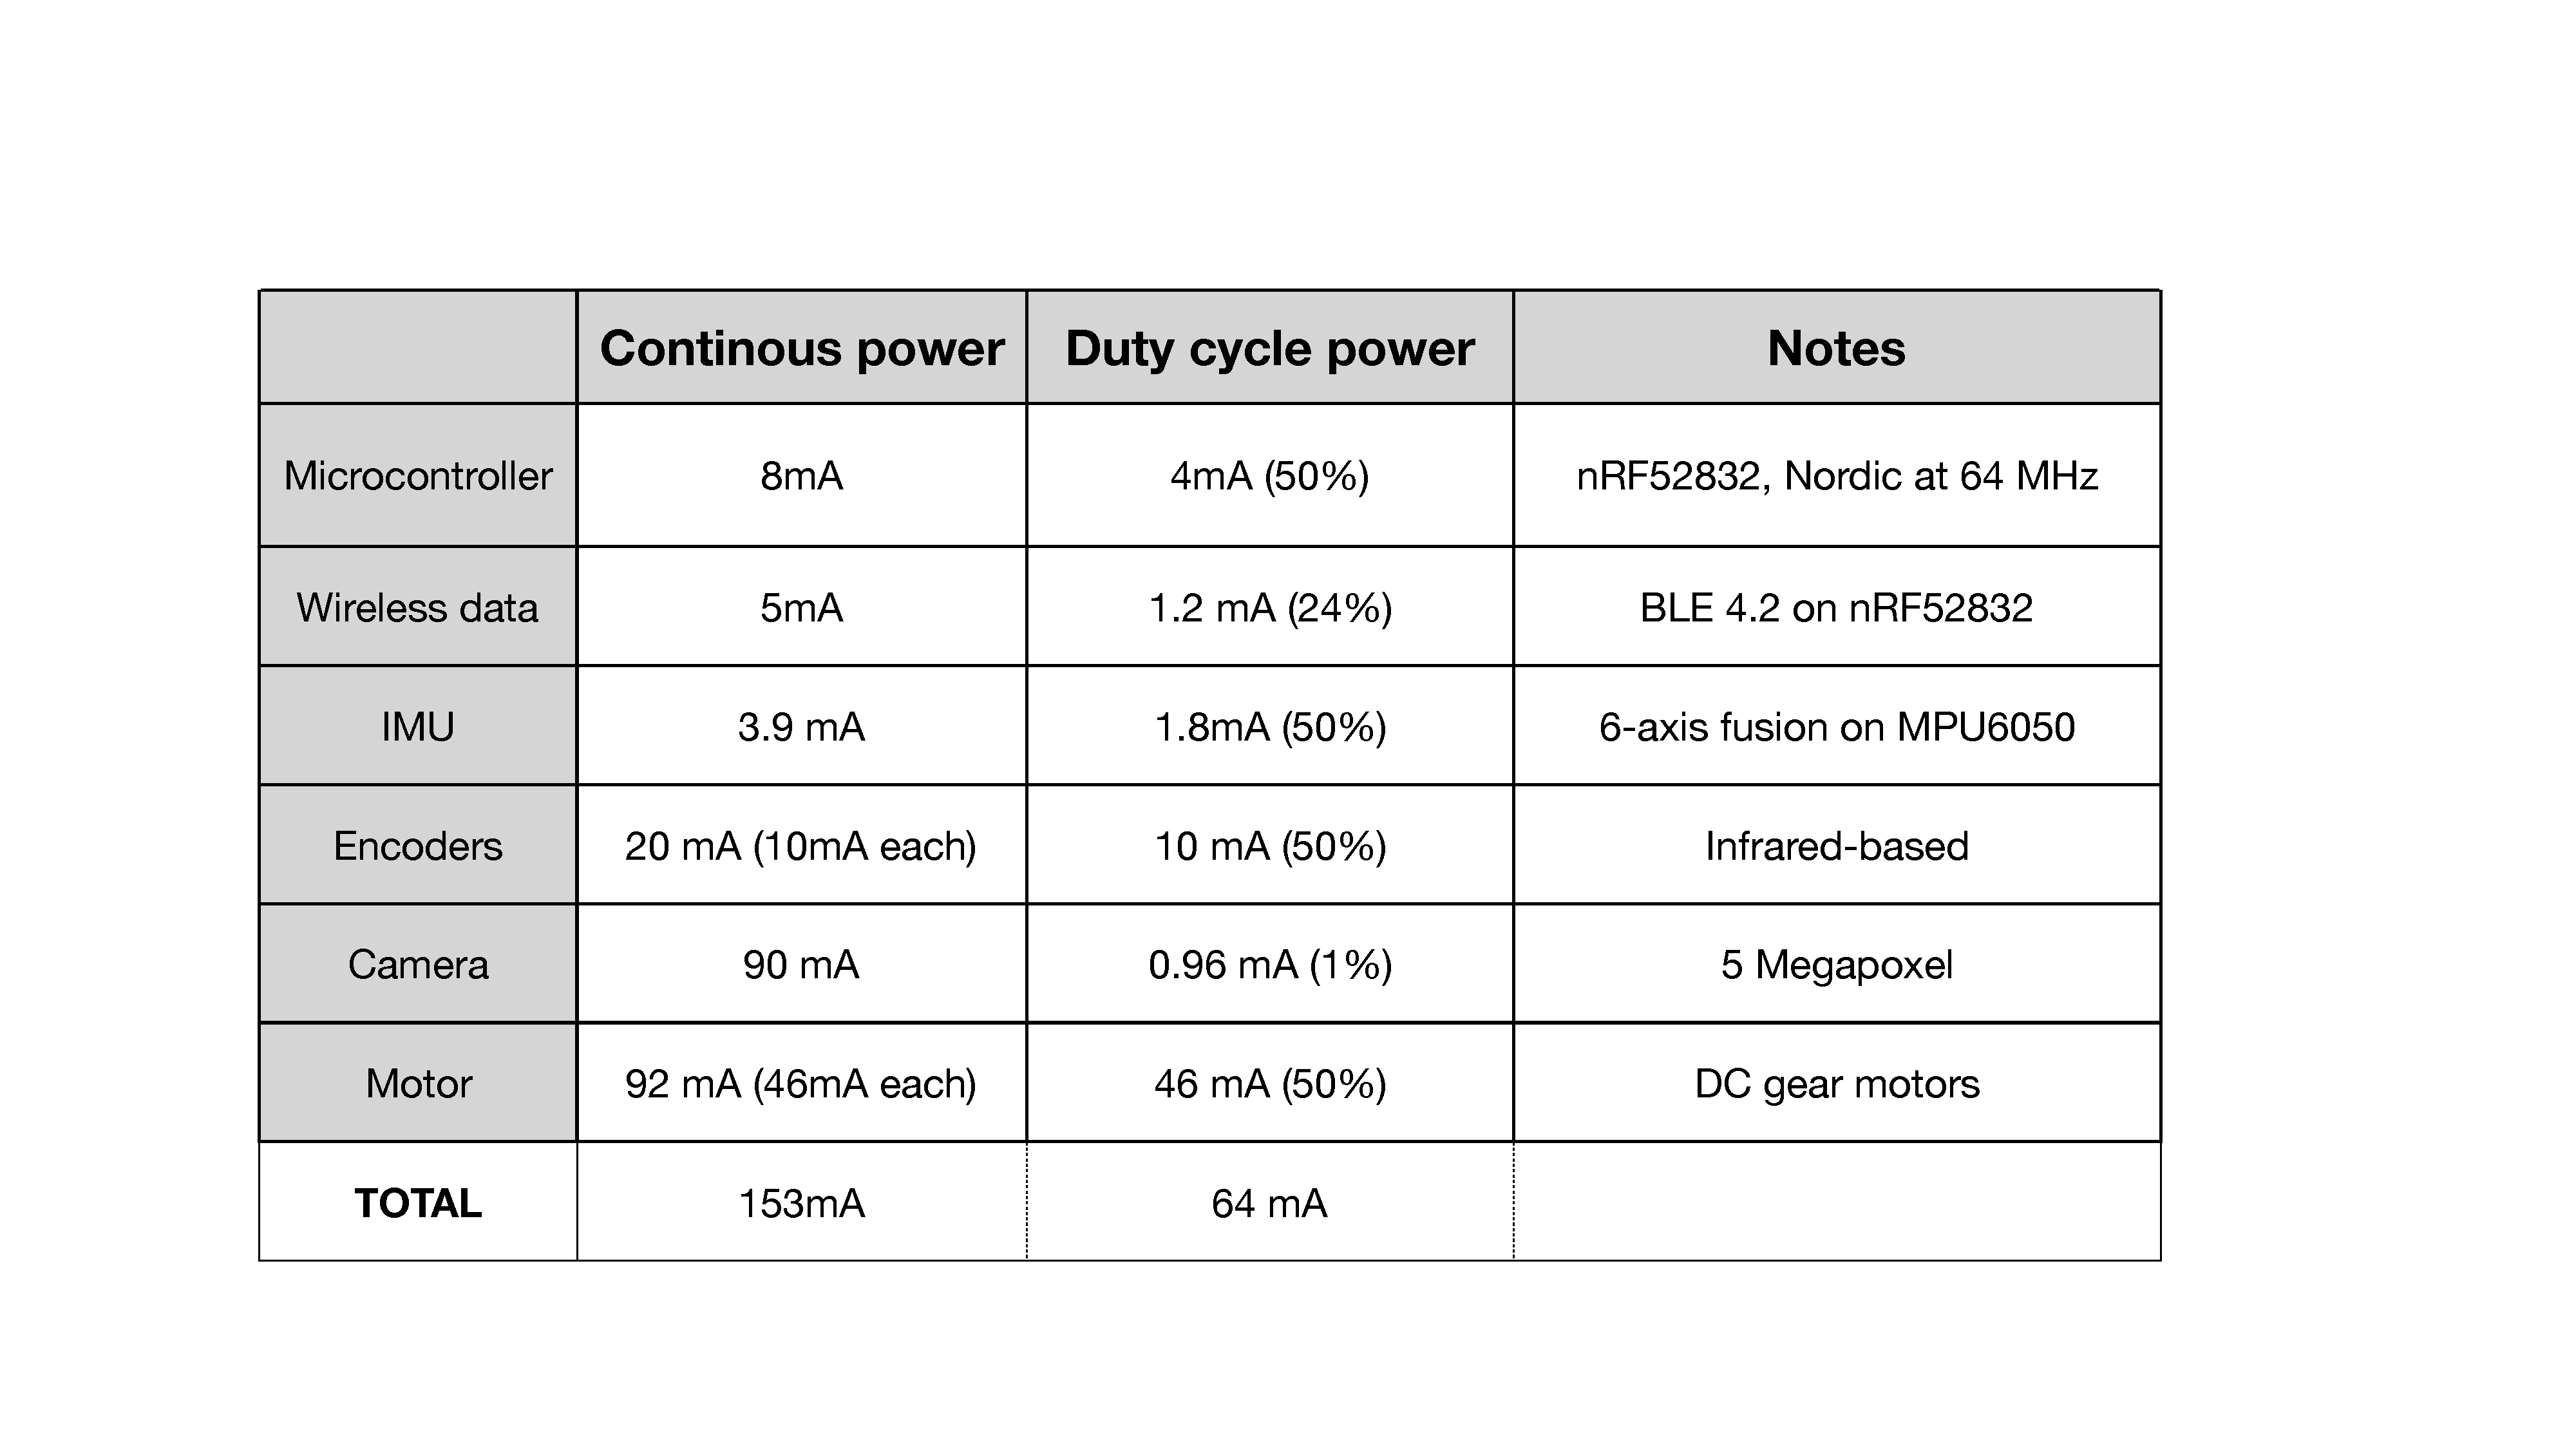
\includegraphics[width=14.0cm]{pictures/power_consumption_pics/power_graph.pdf}
\caption{Table showing current consumption of different robot subsystems. }
\label{fig:power_con_compare}
\end{figure}

\section{Summary}
The motors consume more than 2/3rd of the energy. It is an area where it is difficult to optimize. Vertical climbing requires significant energy expenditure, even with high efficiency of electrical motors. Fundamentally to move 30-gram robot 1-meter vertically requires 0.3Joules of energy or 0.03mA. This estimate does not account for overhead such as friction and motor efficiency, which can be significant. %Considering that the efficiency of brushed gear motors is about 50\%, the energy is 0.06mA.  

The camera provides an engineering challenge for integration into the robot because of large power consumption and data rate. I believe it is possible to integrate an off-the-shelf camera. Previous research has shown that a camera can be powered with RFID~\cite{naderiparizi2015wispcam}. Furthermore, low-resolution optical sensors with custom image processing chips (e.g., optical mouse sensor) could be used to allow better integration. 


